\documentclass[runningheads]{llncs}

\usepackage[T1]{fontenc}
\usepackage{graphicx}
\usepackage[top=3cm, bottom=3cm, left=3.5cm, right=3.5cm]{geometry}
\usepackage{csquotes}
\usepackage[english]{babel}
\usepackage[T1]{fontenc}
\usepackage{ragged2e}
\usepackage{amsfonts}
\usepackage{systeme}
\usepackage{amsmath}
\usepackage{amssymb}
\usepackage{comment}
\usepackage{multicol}
\usepackage{lipsum} 
\usepackage{graphicx}
\usepackage{stmaryrd}
\usepackage{systeme}
\usepackage{wrapfig}
\usepackage{colortbl}
\usepackage{cellspace}
\usepackage{stmaryrd}
\usepackage{ntheorem}
\usepackage{lmodern}
\usepackage{mathtools}
\usepackage{ragged2e}
\usepackage{tabularx}
\usepackage{fancyhdr}
\usepackage{caption}
\usepackage{xcolor}                             % pour les couleurs
\usepackage[linkbordercolor=white]{hyperref}    % après avoir chargé xcolor
\usepackage{systeme}
\usepackage[T1]{fontenc}
\usepackage{lmodern}
\usepackage{listings}
\usepackage{tikz}
\usepackage{mdframed}
\usepackage{xparse}
\usepackage{booktabs}
\usepackage{adjustbox}
\usepackage{float}
\usepackage{enumitem}
\usepackage{tcolorbox}
\usepackage{fancyvrb}
\usepackage{tikz-cd} 
\usepackage{amsmath}
\usepackage{mathrsfs}  
\usepackage{amssymb}
\usepackage{tkz-graph}
\usepackage{caption}
\usepackage{multicol}
\usepackage{listings}                           % Importation du package listings
\usepackage{xcolor}                             % Pour ajouter de la couleur
\usepackage{acronym}
\usepackage[ruled,vlined,linesnumbered,english]{algorithm2e}

% If you use the hyperref package, please uncomment the following two lines
% to display URLs in blue roman font according to Springer's eBook style:
%\usepackage{color}
%\renewcommand\UrlFont{\color{blue}\rmfamily}
%\urlstyle{rm}

\begin{document}

\title{Cross-disciplinary applications of the Toulbar2 solver}
%
%\titlerunning{Abbreviated paper title}
% If the paper title is too long for the running head, you can set
% an abbreviated paper title here
%
\author{Hugo Garcia\inst{1} \and
Philippe Gauthier\inst{1} \and
Marco Sanfilippo\inst{1} \and
Mathis Francine-Habas\inst{1} \and
Martin Cooper\inst{2}\thanks{Research director}\orcidID{0000-0003-4853-053X}}

\authorrunning{H. Garcia et al.}

\institute{University of Toulouse, 118 Narbonne road 31062 Toulouse, France\\
\email{\{hugo.garcia, philippe.gauthier, marco.sanfilippo, mathis.francine-habas\}@univ-tlse3.fr} \and
Toulouse Institute of Computer Science Research, Cr Rose Dieng-Kuntz 31400 Toulouse, France\\
\url{https://www.irit.fr/departement/intelligence-artificielle/adria/}}

\maketitle

% ==================================================================================================================================
% PARTIE 0 : Abstract

\begin{abstract}
    The valued constraint satisfaction problem (VCSP) or weighted constraint satisfaction problem (WCSP) is a problem of finding an assignment of minimal cost to a set of variables given soft and hard constraints and is solved using a branch-and-bound search (BnB). By finding a good lower bound to a given instance, subtrees of the BnB can be quickly pruned to efficiently find an optimal solution. The solver Toulbar2 uses many different techniques to find such lower bounds. This paper studies the cross-disciplinary application of the solver Toulbar2, ranging from solving difficult combinatorial problems, to real-world application such as bioinformatics and resource management and finally artificial intelligence. In many cases where the problem was able to be written using the VCSP framework, Toulbar2 was able to outperform other state-of-the-art solvers.

    \keywords{Toulbar2 \and VCSP \and Protein design \and Operations Research \and AI}
\end{abstract}

% ==================================================================================================================================
% PARTIE 1 : Introduction

\section{Introduction}

The \ac{CSP} involves finding an assignment for a set of variables over a finite domain that respects a set of given hard constraints. 
To find a solution for a \ac{CSP}, backtracking search is used which will assign values to variables and create a new subtree at each step. Once the current instance is infeasible, the algorithm will backtrack and continue with a different assignment until a solution to the original problem is found. However, many real-world problems require optimization rather than mere satisfaction.

The \ac{VCSP} or \ac{WCSP} is considered a generalization of the classic \ac{CSP}. 
In a \ac{VCSP}, a \ac{CFNs} framework is used. \ac{CFNs} are a tuplet consisting of a finite set of discrete variables $X$, a finite domain $D$, a finite set of soft or hard constraints $C$ and a maximum cost $k$. Soft constraints assign a cost to a specific assignment of a subset of variables. The NP-Hard problem of the \ac{VCSP} is to find the instantiation of minimal cost. 

To solve a \ac{VCSP}, the \ac{BnB} algorithm is used. \ac{BnB} explores the solution space by ``\textit{branching}'' : like for CSP, it assigns a value to a variable and creates a new subtree each time. At any node, if the current instance has cost higher than maximum cost k or its cost is higher than the cost of the best solution found so far, the branch is pruned and the search backtracks. This process continues until all branches have been pruned, and the best global solution is found.
\begin{figure}[H]
    \centering
    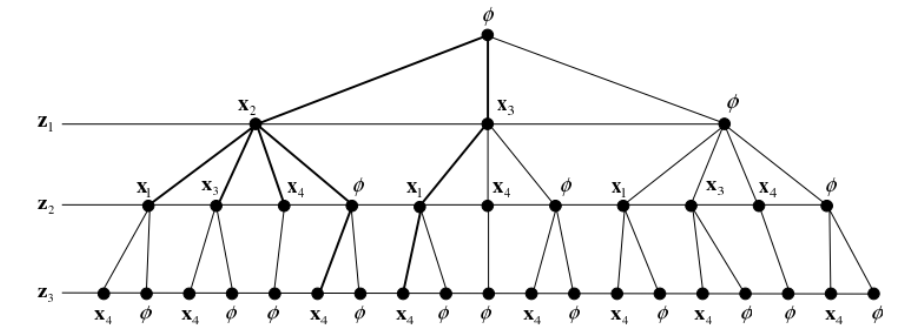
\includegraphics[width=8cm]{images/bnb.png}
    \caption[Example of \ac{BnB} : Mobile Robot Localisation and Mapping in Extensive Outdoor Environments.]{\textbf{Example of \ac{BnB} : Mobile Robot Localisation and Mapping in Extensive Outdoor Environments.}\cite{mobile_robot_localisation_mapping_extensive_outdoor_environments}}
\end{figure}

The efficacy of the branch-and-bound algorithm depends on the lower bound available. 
In a Cost Function Network, functions are categorized by their arity : unary functions (arity 1) assign a cost to individual variable assignments, binary functions (arity 2) assign a cost to pairs of variables and the nullary constant (arity 0), denoted as $c_{\emptyset}$, is the starting cost of the problem. Therefore, the nullary constant also represents a global lower bound on the cost of any complete assignment.

\ac{EPTs} transfer costs from one constraint to another while preserving the same optimal solution for the problem. Below, three different \ac{EPTs} are presented for an example with three variables $(x, y, z)$ with two possible assignments $(a, b)$. A line joining two values represents a cost of $1$ for this assignment in the corresponding binary cost function. Unary costs are represented as numbers inside the different assignments and the nullary constant is shown above.
\begin{figure}[H]
    \centering
    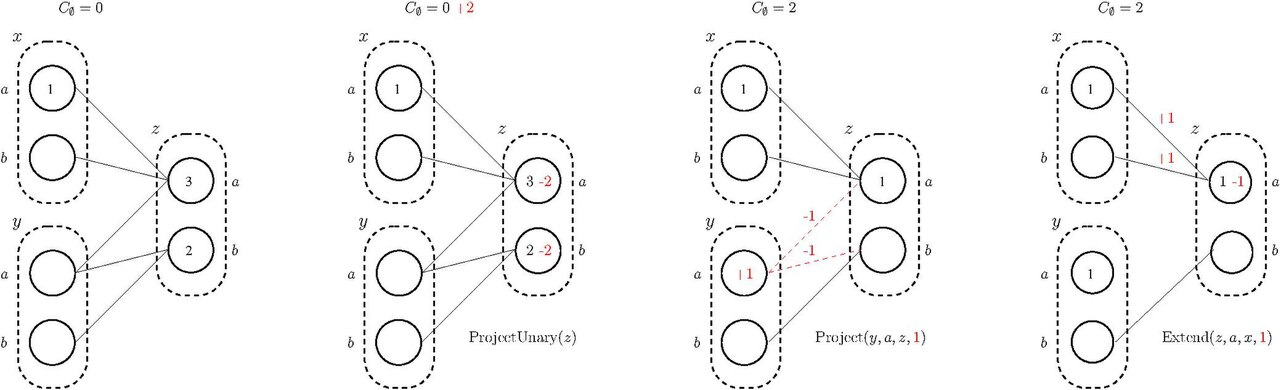
\includegraphics[width=12cm]{images/ept.jpg}
    \caption[Basic Equivalence Preserving Transformations]{\textbf{Basic Equivalence Preserving Transformations.}\cite{npariscril_ept_2012}}
\end{figure}

By successive \ac{EPTs}, the cost can be shifted and concentrated into the nullary constraint $c_{\emptyset}$, thus giving a better lower bound for the \ac{VCSP}. This new lower bound allows the solver to quickly prune subtrees.

This process of applying successive \ac{EPTs} to obtain a better lower bound is known as \ac{SAC}. Different inference techniques to obtain a good lower bound exist, and those include the following : \ac{FDAC}, \ac{EDAC}, \ac{VAC} and \ac{OSAC}. Those inference techniques vary in relative strength vs relative computational cost, but generally the better the lower bound found, the higher the computational cost becomes. \ac{OSAC} provides the best lower bound, followed by \ac{VAC}, then \ac{EDAC} and finally \ac{FDAC}.

These theoretical findings are used in the solver Toulbar2. Toulbar2 is an open-source \textit{C++} solver for discrete optimization problems within the cost function network framework. The solver integrates \ac{SAC} operations, dynamically switching and choosing the best inference technique at a given node, and uses a branch-and-bound search to quickly explore the solution space and find the optimum. This document provides a state-of-the-art review of the solver’s cross-disciplinary impact. We begin by examining the solver’s ability to solve difficult combinatorial computer science problems against other state-of-the-art solvers, then explore their real world applications ranging from structural bioinformatics to classic operations research problems and finally discuss their recent integration into neuro-symbolic artificial intelligence networks.

% ==================================================================================================================================
% PARTIE 2 : Algorithmic Foundations & Solver Development

\section{Combinatorial problem solving}

Toulbar2 has been tested for solving many challenging combinatorial problems using a \ac{CFNs} framework and often outperformed other powerful state-of-the-art solvers.
Below will be some examples of such problems.

\subsection{An application to graph theory and the cluster editing problem}
Zahn's decision problem can be described as the cluster editing problem. Given a graph, what is the minimal number of operations (adding edges, removing edges) needed to create a disjoint union of cliques. The \ac{ZP} is generally an NP-hard problem.
In a paper titled ``A constraint programming approach to the Zahn’s decision problem''\cite{amel_constraint_2014}, the \ac{ZP} was transformed into a valued constraint satisfaction problem. This transformation is done as follows : 

\begin{itemize}
    \item A boolean variable is added for each pair of vertices. When a variable is set to true by the solver, then the decision is to keep or add the edge between the vertices. Else, the decision is to remove or not add an edge between the two vertices.
    \item A unary soft constraint is added for each variable. The cost of assigning $0$ to a variable $x$ is $1$ if the edge exists in the original graph, and 0 otherwise.
    \item A ternary hard constraint is added for each pair of $3$ edges which together creates the subgraph $P3$ described in the figure below. These ternary hard constraints are added to ensure that the resulting graph is a disjoint union of cliques. This result comes from the fact that a disjoint union of cliques cannot contain a subgraph isomorphic to $P3$, as explained in the paper.
\end{itemize}

\begin{figure}[H]
    \centering
    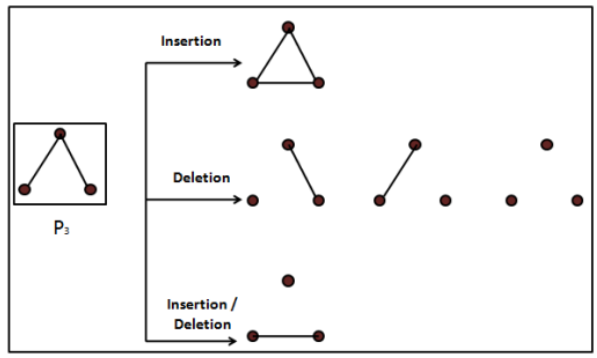
\includegraphics[width=0.4\textwidth]{images/ZP.png}
    \caption[$P3$ Graph and insertion/deletion possibilities.]{\textbf{$P3$ Graph and insertion/deletion possibilities.}\cite{amel_constraint_2014}}
\end{figure}

Using Toulbar2 to solve the \ac{VCSP}, the results found were much better than the fixed parameter algorithm for cluster editing presented before. The \ac{VCSP} algorithm performed better on both sparse and dense graphs. These results show the efficacy and utility of the constraint programming paradigm for general graph related problems.

\subsection{Constraint programming for calculating partition functions and discrete integration in high dimensions}

Discrete integration in high dimensions is considered to be a generally unsolved and difficult problem, is typically \#P-Hard and has applications to a wide variety of fields. This difficulty arises from the phenomenon known as the curse of dimensionality. In the paper ``Taming the Curse of Dimensionality : Discrete Integration by Hashing and Optimization``\cite{ermon_taming_2013}, reduces the task of discrete integration into a collection of \ac{MAP} sub-problems, which are NP-Hard instead.

The main challenge involves calculating the partition function. A partition function is a sum of all possible configurations of a set $X$ where $w(x)$ is a weight function assigning a weight to a configuration.

\begin{equation}
    Z = \sum_{x \in \mathcal{X}} w(x)
\end{equation}

A commonly known example in physics is the Boltzmann distribution, a probability distribution that describes the likelihood of a system being in a specific configuration. The corresponding partition is as follows :

\begin{equation}
    w(x) = e^{-\frac{E(x)}{k_B T}} 
    \qquad \text{and} \qquad 
    Z = \sum_{x \in \mathcal{X}} e^{-\frac{E(x)}{k_B T}}
\end{equation}

\begin{itemize}
    \item $E(x)$ : The total energy of the configuration $x$.
    \item $k_B$ : The Boltzmann constant.
    \item $T$ : The absolute temperature.
\end{itemize}

A partition function can also be understood as a discrete integral, and is a computational task that is intractable due to the exponential number of configurations. WISH is a randomized algorithm which bypasses this challenging problem by solving, like said above, a collection of NP-Hard problems instead.

Using the state-of-the-art combinatorial tool Toulbar2 to solve the \ac{MAP} queries, WISH provided a constant-factor approximation of discrete integrals with high probability, that could since then only be handled heuristically. Another significant advantage of this approach is that these independent optimization instances can be solved in parallel. 

These results show the impact of Toulbar2 when a difficult \#P problem is reduced to a combinatorial problem that can be solved with constraint programming. The wide applications of discrete integrations demonstrate the utility of the \ac{VCSP} solver.

\subsection{Toulbar2 for the weighted $N$-queen and quadratic assignment problems}

The $N$-Queen problem is a non-trivial mathematical problem that looks for a placement of $N$ queens on board of chess of size $N$ by $N$ where no two queens are threatening each other. The figure below shows an example of a solution where $n = 8$.

\begin{figure}[H]
    \centering
    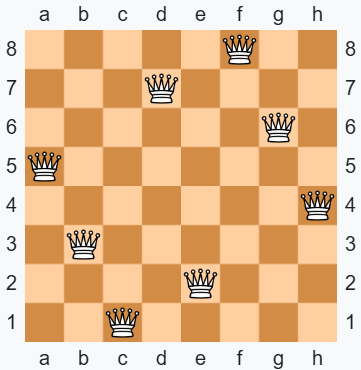
\includegraphics[width=4cm]{images/nqueens.png}
    \caption[Example of a solution for the $N$-queen problem]{\textbf{Example of a solution for the $N$-queen problem with $n=8$} \cite{nquennsproblem}}
\end{figure}

The weighted $N$-Queen problem is a difficult optimization problem where every queen placement incurs a cost, and the goal is to find the lowest cost solution. 

A key advancement by Sewa et al. (2022)\cite{traore_new_2013} improved the Toulbar2 performance by integrating a more powerful way to propagate ALLDIFFERENT constraints for \ac{SAC}. An ALLDIFFERENT constraint is a constraint where no two variables can have the same value. By modeling the cost as a unary constraint and using three ALLDIFFERENT constraints for the column, diagonal and anti-diagonal uniqueness, the upgraded version of Toulbar2 significantly outperformed other state-of-the-art solvers for the $N$-Queen problem.

Furthermore, with this new improved version of Toulbar2, the authors also tested its performance for the quadratic assignment problem (QAP). The QAP is a difficult NP-Hard problem where we seek to assign $n$ facilities to $n$ locations so as to minimize the total cost which is determined by the flow between facilities and the distance between locations. The results found that toulbar2 returned the highest quality solution with a gap of $3.9\%$ to the best known decision.

These examples show the relevance of Toulbar2 when paired with a new propagator against state-of-the-art solvers for difficult NP-Hard combinatorial problems.

\subsection{Toulbar2 application for the knapsack problem with a conflict graph and computational protein design}

The knapsack problem is a classic NP-hard problem in combinatorics and computer science goes as follows : given a maximum weight capacity $C$, a set of objects each an assigned $weight$ and $value$, what is the set of objects that maximize the value while respecting the weight capacity.

The \ac{KPCG} is a variant of the knapsack problem where conflict between objects is added. For a given graph $G$, each object is assigned to a vertex. An edge between vertex $i$ and $j$ implies that object $i$ and $j$ cannot be in a solution together. The \ac{KPCG} is difficult to solve with constraint programming as \ac{CFNs} do not allow the modeling of linear constraint without a non-trivial performance penalty, especially those with large coefficients.

Montalbano et al. (2022)\cite{montalbano_multiple-choice_2022} developed a way to model pseudo boolean linear constraints with \ac{CFNs} allowing more problems to be solved using \ac{VCSP}. When toulbar2 was compared with the state-of-the-art \ac{ILP} solver \textit{CPLEX 20.1} for solving the \ac{KPCG}. The approach was evaluated across six distinct classes of the \ac{KPCG}, each having $720$ instances with varying capacities, weight distributions, and profit correlations. The results found that Toulbar2 was more efficient than \textit{CPLEX} in $4$ out $6$ classes. Furthermore, Toulbar2 found the best solutions for the largest number of instances in every class.

\begin{figure}[H]
    \centering
    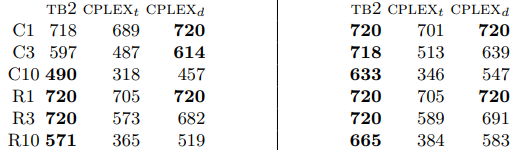
\includegraphics[width=0.5\textwidth]{images/resultat_knapsack.png}
    \caption[Number of solved instances and number of times a solver found the best solution within the time limit for six different classes of \ac{KPCG}.]
        {\textbf{Number of solved instances (left) and number of times a solver found the
        best solution within the time limit (right) for six different classes of \ac{KPCG}.} Cplex was tested with two different encodings : tuples ($t$) and direct ($d$).\cite{montalbano_multiple-choice_2022}}
\end{figure}

This new technique also helped model the protein design problem, which is one of the main applications of the Toulbar2 solver, as it will be shown in the following section.

% ==================================================================================================================================
% PARTIE 3 : Protein

\section{Bioinformatics \& Life Sciences}

Protein design \ac{CMD} involves creating artificial proteins capable of adopting a given structure and performing a specific function. This field is highly important because it enables the design of more efficient enzymes, biological sensors, or even nanoscale structures.

A central aspect is the control of \acp{PPI}. In cells, proteins do not act alone: they assemble into organized complexes. For example, some proteins form regular structures composed of multiple identical copies (homomers), while others combine several different proteins (heteromers). Being able to switch from a homomeric system to a heteromeric one would allow the creation of much more complex and controlled assemblies.

However, designing a protein is very challenging. For a given structure, there is an enormous number of possible sequences. Moreover, each sequence can adopt multiple conformations\footnote{The $3D$ shape a protein takes when it folds, which determines how it functions.}. This creates a vast search space.
To simplify, classical methods make two important assumptions :

\begin{itemize}
    \item The backbone is rigid (the overall structure does not move) ;
    \item Only the side chains change, in the form of rotamers\footnote{A specific orientation of a part of a protein, often a side chain, which can rotate around a bond, giving several possible discrete positions.}.
\end{itemize}

With these simplifications, the problem can be seen as an optimization task : finding the combination of rotamers that yields the lowest energy. Nevertheless, the problem remains very complex (NP-hard).
Over time, different approaches have been developed : physical methods, exact methods, deep learning, and then hybrid approaches. The objective has always been the same: to find a good compromise between accuracy, speed, and control.

\subsection{Formalization and Classical Methods of Protein Design}

\ac{CPD} is generally formulated as an optimization problem : the goal is to identify the amino acid sequence that minimizes the protein’s energy, called the \ac{GMEC}. 
This energy is minimized because, naturally, a protein adopts its most stable conformation, i.e., the one with the lowest energy.

\begin{figure}[H]
    \centering
    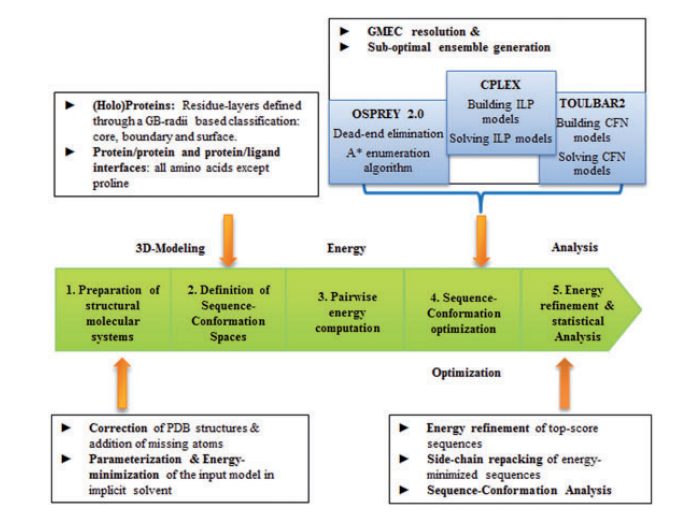
\includegraphics[width=0.6\textwidth]{images/schema_framework-CPD_partie1.png}
    \caption[Flow chart of the \ac{CPD} framework]{\textbf{Flow chart of the \ac{CPD} framework.}\cite{traore_new_2013}}
\end{figure}

In this framework, each position of the protein can adopt different rotamers (local conformations of side chains). The total energy of the protein is calculated as the sum of local contributions (energy of a single residue) and pairwise interactions between residues. The problem thus consists of selecting a rotamer for each position in order to minimize this global energy.

The problem quickly becomes combinatorial : if each position can take multiple rotamers, the total number of possible combinations grows exponentially with the size of the protein. To address this, two main families of methods have been developed :

Heuristic methods :

\begin{itemize}
    \item Monte Carlo, simulated annealing ;
    \item Genetic algorithms.
\end{itemize}

These methods explore the solution space quickly, but they can become trapped in local optima and do not guarantee finding the global solution.

Exact methods :

\begin{itemize}
    \item Dead-End Elimination (DEE) ;
    \item $A^*$ search ;
    \item Integer Linear Programming (ILP).
\end{itemize}

These approaches guarantee finding the optimal solution according to the energy model, but their computational cost is often high, especially for large proteins.

A crucial point is that the calculated optimal solution is not necessarily the best in practice, because the energy models used are approximate. For this reason, it is common to also examine solutions that are close to the optimum.
This formalization provides a rigorous framework for protein design, but it relies on significant simplifications, notably the rigidity of rotamers and the approximation of energies. Furthermore, the computational cost grows rapidly with protein size, which limits direct applicability to large structures.

\subsection{Advanced Exact Approaches and Problem Analysis}

To improve the efficiency of exact methods in protein design, the problem has been reformulated in terms of constraints. This allows leveraging more structured and systematic optimization techniques.

Computer-aided protein design can be represented as a \ac{CFNs} :

\begin{itemize}
    \item Each residue corresponds to a variable ;
    \item Each rotamer represents a possible value for that variable ;
    \item Each interaction between residues is encoded as a cost.
\end{itemize}

The objective is then to find the combination of values (rotamers) that minimizes the total cost of the system.

In the \ac{CFNs} framework, there is a clear mapping from the protein structure to a constraint graph : residues become nodes, interactions define edges with associated costs. This mapping highlights how structural information is transformed into a formal optimization problem.

The Toulbar2 solver is commonly used to tackle this formulation. It applies techniques such as Branch and bound, which explores the solution space intelligently or Pruning, which eliminates infeasible or suboptimal solutions early.

These capabilities allow the solver not only to identify the exact \ac{GMEC} but also to enumerate multiple near-optimal solutions. Such solutions are particularly useful for analyzing the fitness landscape of the protein: some problems are simple, exhibiting a single global minimum, others are more complex, with many local minima creating a rugged landscape.

\begin{figure}[H]
    \centering
    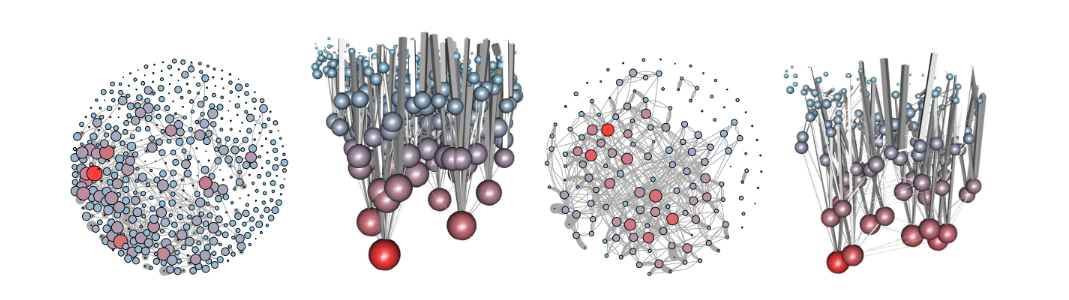
\includegraphics[width=11cm]{images/schema_soft_rought_landscapee_partie2.png}
    \caption[Local optima network with basin edges for $2ckx$ and $2gkt$ in $2D$ and $3D$ representations.]{\textbf{Local optima network with basin edges for $2ckx$ (left side) and $2gkt$ (right side) in $2D$ and $3D$ representations.} The
size is the log of the basin of attraction size. The color is the fitness : the better, the warmer. The thickness of the edges is
proportional to the probability of passing from one basin to the other.\cite{simoncini_fitness_2018}}
\end{figure}

Understanding this landscape is crucial, as it explains why certain optimization methods perform well in some cases but struggle in others.

To further improve computational performance, techniques like \ac{LNS} are employed: only a portion of the protein is modified at a time. This subset is then optimized exactly while keeping the rest fixed.

\ac{CFNs}-based approaches with Toulbar2 enable more efficient exact optimization and provide deeper insight into the structure of the problem. Nevertheless, they remain constrained by the size of the protein system and the simplifications inherent in the energy and rotamer models.

\subsection{Deep Learning and Hybrid Approaches}

Deep learning has recently transformed the field of protein design, providing new ways to predict and generate sequences compatible with a given structure.
Models such as \textit{ProteinMPNN} learn directly which sequences are compatible with a target structure, enabling the rapid generation of realistic proteins.

However, these models have limitations :

\begin{itemize}
    \item They are difficult to control precisely ;
    \item They struggle to handle complex constraints effectively.
\end{itemize}

A particularly challenging problem is multi-state design, where the goal is to :

\begin{itemize}
    \item Favor a desired interaction (e.g., $AB$) ;
    \item Avoid undesired interactions (e.g., $AA$ or $BB$).
\end{itemize}

\begin{figure}[H]
    \centering
    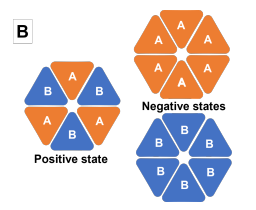
\includegraphics[width=0.35\textwidth]{images/schema_positive_negativestate_partie3.png}
    \caption[Designing orthogonal component with the same fold requires explicitly accounting for negative homomeric states]{\textbf{Designing two orthogonal
components with the same fold requires explicitly representing the two undesirable homomeric negative states
on the right.}\cite{dessaux_designing_2024}}
\end{figure}

Classical deep learning models often struggle with multi-state design because they must simultaneously satisfy conflicting objectives.

To address this, a hybrid approach has been developed, combining deep learning and exact optimization :

\begin{itemize}
    \item Effie : a deep learning model that produces a scoring function for candidate sequences ;
    \item Toulbar2 : an exact solver that optimizes this scoring function under explicit constraints.
\end{itemize}

\begin{figure}[H]
    \centering
    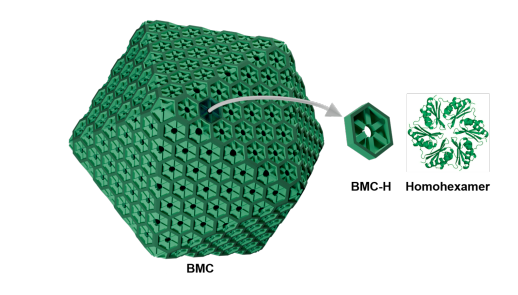
\includegraphics[width=0.5\textwidth]{images/schema_bmc_partie3.png}
    \caption[BMC-H homohexamer of bacterial microcompartment shell.]{\textbf{BMC-H homohexamer of bacterial microcompartment (BMC) shell.}\cite{dessaux_designing_2024}}
\end{figure}

This combination allows better control over specific interactions, simultaneous management of multiple states, and generation of sequences with improved overall quality.

Experimental and simulation results demonstrate that this approach performs better in computational simulations and has been validated experimentally, showing real interactions and measurable fluorescence.

Hybrid approaches leverage the strengths of both deep learning and exact methods. They provide more precise control over protein design and multi-state objectives, although they remain computationally more demanding.


Protein design has undergone significant evolution over the years :

From physical methods to exact approaches, then to deep learning, and finally to hybrid strategies.

Each approach has brought improvements, but also comes with inherent limitations.

The main remaining challenges include :

\begin{itemize}
    \item Protein flexibility, as rigid backbone approximations remain oversimplified.
    \item Accuracy of energy or scoring models, which can limit the reliability of predictions.
    \item Scalability, i.e., the ability to handle large and complex protein systems efficiently.
\end{itemize}

Hybrid approaches currently appear the most promising, as they combine precision, explicit control, and the ability to manage complex constraints.This is particularly valuable for designing specific interactions and multi-state systems.

% ==================================================================================================================================
% PARTIE 4 : Resource Management & Planning

\section{Resource Management \& Planning}

Although the Toulbar2 solver has gained a strong reputation in the field of bioinformatics, 
the Cost Function Networks formalism is proving particularly well-suited to classical operational research problems. 
The management and allocation of resources generally involve satisfying strict rules (hard constraints) 
whilst optimising quality criteria or preferences (soft constraints). 
This section illustrates how soft local consistency algorithms (such \ac{OSAC} \& \ac{EDAC}) implemented in Toulbar2 
enable the resolution of industrial-scale planning problems, whilst highlighting the strengths and limitations 
of these exact approaches compared to other paradigms such as \ac{MILP}.

\subsection{Spatio-temporal allocation and conflict management}

Planning and allocating physical resources often require merging two complex dimensions : space and time. 
This could mean rotating crops across agricultural land over several years. It could also involve coordinating 
flight paths in restricted airspace. These problems require satisfying strict rules while simultaneously optimizing quality criteria.

This subsection illustrates how the \ac{WCSP} formalism models these spatio-temporal environments. 
It also evaluates the efficiency of the Toulbar2 solver compared to other exact methods.

The crop allocation problem consists of assigning different crop types (the values) to agricultural plots (the variables) over a finite time horizon. 
The approach proposed by Akplogan et al. (2013)\cite{akplogan_solving_2013} stands out by simultaneously modeling spatial and temporal constraints at the farm level.

The model integrates two types of constraints :

\begin{itemize}
    \item \textbf{Hard constraints :} These guarantee agronomic feasibility. Examples include the minimum return time for a crop on the same plot, or respecting the biophysical properties of the soil.
    \item \textbf{Soft constraints :} These reflect the farmer's preferences. Examples include the spatio-temporal balance of the crops, or the beneficial effects of previous crops on the soil.
\end{itemize}

\begin{figure}[H]
    \centering
    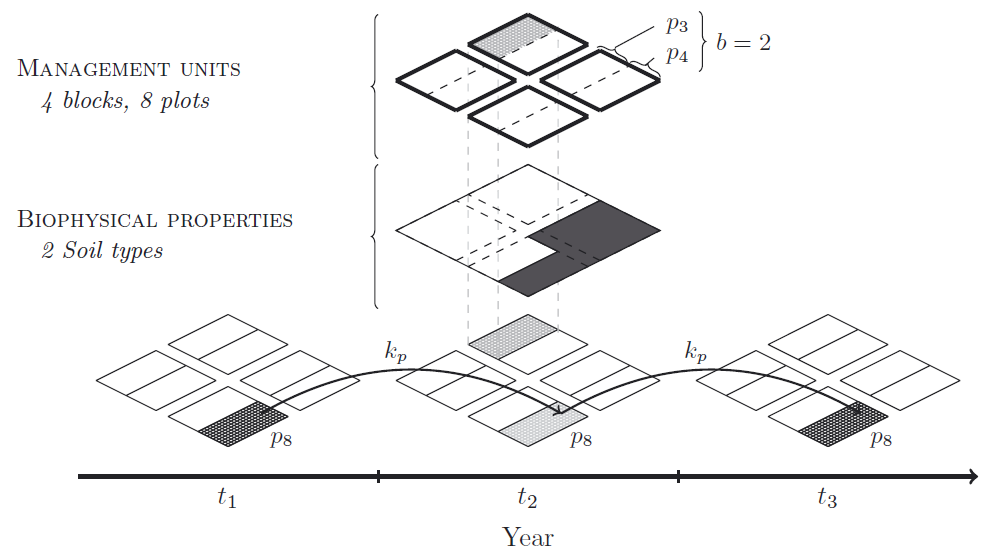
\includegraphics[width=9cm]{images/crop_allocation_explication.png}
    \caption[Schematic representation of the spatial and temporal aspects of the decision–making problem]{\textbf{Schematic representation of the spatial and temporal aspects of the decision–making problem} ($t_i$ : year, $b$ : block, $p_j$ : plot, $k_p$ : preceding effect).\cite{akplogan_solving_2013}}
\end{figure}

To solve this problem, the authors compared two approaches. The first is a \ac{WCSP} formulation solved by Toulbar2. The second is a \ac{MILP} reformulation solved by 
SCIP\footnote{For \ac{MIP} and \ac{MINLP}, SCIP is now among the quickest non-commercial solvers. 
Additionally, it is a framework for branch-cut-and-price and constraint integer programming.}.

On a theoretical level, this study highlights a link with local consistency algorithms. The continuous relaxation of the \ac{MILP} corresponds to the dual problem of the \ac{LP} encoded by \ac{OSAC}.
When the upper bound is infinite, this relaxation is theoretically stronger than the \ac{EDAC} consistency used by default in Toulbar2. However, if this upper bound decreases to a finite value, the two algorithms become incomparable.

However, the experiments reveal a major limitation of WCSP-based methods in this specific context. On real-world instances corresponding to medium and large farms, the SCIP solver 
proved nearly three times faster than Toulbar2. Furthermore, it consumed significantly fewer computational resources.

This study demonstrates a clear conclusion. WCSPs offer excellent flexibility for modeling complex spatio-temporal constraint networks. However, on large-scale, pure scheduling problems, 
the Toulbar2 solver faces real competition from classic \ac{MILP} solvers.
\medskip{10cm}


In a much more dynamic spatio-temporal context, Schmidt et al. (2020)\cite{chaboud2020tackling} apply the \ac{WCSP} formalism to air traffic conflict resolution. A collision risk may be detected between several aircraft. 
When this happens, a generation method called ``Lumberjack'' produces a vast set of discretized alternative trajectories for each plane. The combinatorial challenge is then to select the best combination of compatible flight paths. 
This ensures the conflict is resolved optimally.

\begin{figure}[H]
    \centering
    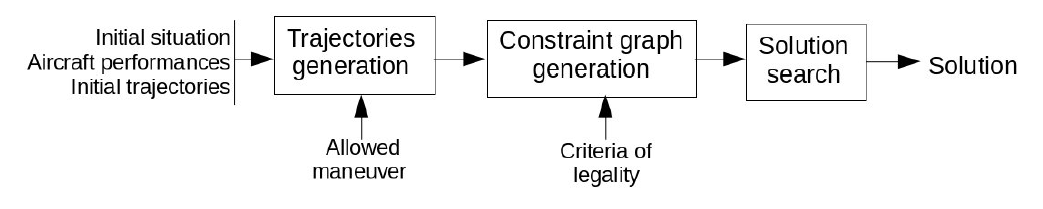
\includegraphics[width=9cm]{images/lumberjack_algo.png}
    \caption[Lumberjack method steps.]{\textbf{Lumberjack method steps.}\cite{chaboud2020tackling}}
\end{figure}

In this model, each aircraft represents a variable of the problem, and the set of its alternative avoidance trajectories constitutes its domain of values.

\begin{figure}[H]
    \centering
    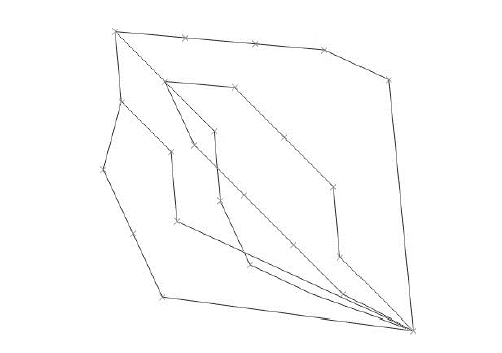
\includegraphics[width=6cm]{images/ex_alternative_fligth.png}
    \caption[Potential trajectories going from upper left to lower right.]{\textbf{Potential trajectories going from upper left to lower right.}\cite{chaboud2020tackling}}
\end{figure}

The study compares the performance of the exact solver Toulbar2 with a custom-built ``\ac{SBF}'' algorithm. Analyzing the results highlights a characteristic trait of the \ac{CFNs} architecture and Toulbar2. 
The solver handles scaling the number of variables perfectly well. It efficiently resolves conflicts involving a relatively high number of aircraft ($6$ to $8$ planes). 
In contrast, the \ac{SBF} approach collapses under these conditions.

However, Toulbar2's memory saturates quickly when given too many possible trajectories per plane. In other words, it struggles if the domain size becomes too large. This issue can be explained by two factors. 
First is the memory cost of representing constraints in extension. Second is the heavy cost of applying local consistency algorithms to very large domains.

\begin{figure}[H]
    \centering
    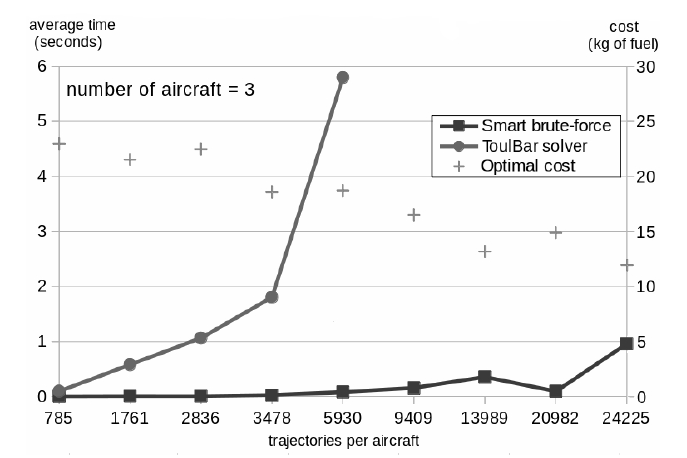
\includegraphics[width=8cm]{images/performance1_SBF_TB2.png}
    \caption[Performance of the two solvers on trajectory generation without greedy algorithms.]{\textbf{Performance of the two solvers on trajectory generation without greedy algorithms.} Average solving time over $100$ tests of the \ac{SBF} (squares) and Toulbar2 (circles) approaches
for instances of a Roundabout with $3$ aircraft, function of the number of generated trajectories
per aircraft. Crosses represent the average cost of the optimal solution.\cite{chaboud2020tackling}}
\end{figure}

To overcome these limitations, the authors highlight a pruning method using a ``greedy'' MinCostMaxClique$^{\ref{algo:mcmc}}$ algorithm. Before launching the exact search, they use a fast, non-optimal greedy heuristic to find an initial valid solution. 
The cost calculated from this solution is then injected into Toulbar2 as an initial ``upper bound''. This trick allows the solver to prune the search tree much faster. 
It removes a considerable number of bad solutions and significantly accelerates the proof of optimality.

\begin{figure}[H]
    \centering
    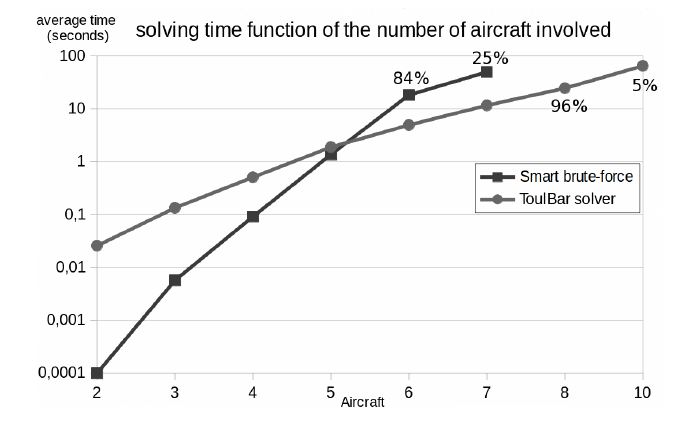
\includegraphics[width=8cm]{images/performance2_SBF_TB2.png}
    \caption[Performance of the two solvers on trajectory generation with greedy algorithms.]{\textbf{Performance of the two solvers on trajectory generation with greedy algorithms.} Average solving time over $100$ tests with statistical noise, of \ac{SBF} (squares) and Toulbar2
(circles) approaches for instances of a Roundabout with approx. $850$ trajectories per aircraft,
function of the number of aircraft involved. When a method does not always succeed before the
$60\text{'s}$ time-out, its success rate is indicated.\cite{chaboud2020tackling}}
\end{figure}

This use case shows that Toulbar2's performance depends heavily on the problem's topology. It also highlights the importance of hybridizing exact methods with fast, non-optimal heuristics. 
This combination guarantees response times that meet real-world industrial requirements.

\subsection{Human resources and global constraints}

Managing space and time is a major challenge. However, human resources planning introduces a different complexity. It requires modeling legal rules and individual preferences.
This subsection highlights how \ac{WCSP} research has had to evolve. It demonstrates the adaptation required to meet the expressivity needed to generate schedules.

Hospital staff scheduling is an optimization problem known for its high combinatorial complexity. In their study, Métivier et al. (2009)\cite{nurse_rostering_problems} apply the \ac{CFNs} formalism and the Toulbar2 solver to generate optimal schedules for nurses. 
Researchers must account for strict staff coverage requirements (hard constraints) as well as staff rest preferences (soft constraints).

The value of this document for this analysis lies in demonstrating the historical limitations of \acp{WCSP} for this type of problem. Historically, \ac{CFNs} were designed around binary constraints. 
However, this type of constraint is poorly suited for modeling human rules. It would require creating an exponentially large constraint network. This makes the solution inefficient.

To overcome this issue, research around Toulbar2 focused on implementing soft global constraints. Unlike a binary constraint, a global constraint simultaneously evaluates a large sequence of assignments. 
For example, a single global constraint can encompass a nurse's entire week or month in a single evaluation.
Métivier et al. (2009) explain how specific algorithms, based on dynamic programming or flow networks, were integrated directly into Toulbar2. This integration allows the application of local consistencies (such as \ac{EDAC}).

This article demonstrates a significant evolution. The \ac{WCSP} paradigm is often associated with structural or biological problems. However, it has now achieved a much richer expressivity.
Integrating soft global constraints into Toulbar2 proves its true capability. This paradigm can now successfully compete with traditional \ac{CP} solvers in the field of human scheduling.

\subsection{Routing and networks}

This final section addresses the allocation of purely abstract and logical resources. The networking and telecommunications field provides an excellent testing ground. It allows us to compare \acp{WCSP} against other major combinatorial optimization standards.

In their study, Lesaint et al. (2014)\cite{lesaint2014developing} examine a complex problem in telecommunications network allocation and configuration : service subscription conflict management. The issue is as follows. A customer may demand a combination of network services that are technically incompatible due to infrastructure limits. 
When this happens, the provider must find the best compromise. This involves downgrading the service or ignoring certain requested options. The goal is to minimize the overall penalty corresponding to customer dissatisfaction.
This NP-hard decision problem was modeled as a \ac{WCSP}.

Instead of isolating Toulbar2, the authors systematically compared the \ac{WCSP} formulation against competing models. These included \ac{MILP} and Partial Weighted Max-SAT. 
The results demonstrate the strength of the \ac{WCSP} approach. By leveraging constraint propagation, it proves highly competitive for dynamically resolving these allocation conflicts.

This operations research use case provides empirical proof. \ac{WCSP} modeling can compete with historically undisputed paradigms like \ac{MILP} or Max-SAT for allocating abstract resources. 
Toulbar2 can sometimes saturate on certain purely linear problems. However, its modeling flexibility and computational power make it an effective alternative for resolving conflicting query satisfaction problems.
\medskip{10cm}


As seen in previous applications, the Toulbar2 solver excels at optimization and planning in deterministic environments. However, resource availability can become uncertain and dynamic. 
A prime example is IoT sensors, whose energy relies on random environmental conditions (Biason et al., 2017)\cite{ieee_transactions_on_mobile_computing}. In these situations, exact planning shows its limitations. 

It then becomes necessary to frame the problem using Markov Decision Processes. Here, Toulbar2 is no longer used as a standalone tool. Instead, it serves as an ``internal computing engine'' powering a probabilistic algorithm.

This need to hybridize exact constraint optimization with models that handle uncertainty marks a natural progression. This question directly drives the integration of \acp{WCSP} into the broader fields of Artificial Intelligence and Machine Learning.

% ==================================================================================================================================
% PARTIE 5 : AI \& Machine Learning

\section{Artificial Intelligence \& Machine Learning}

We have seen that Toulbar2 is a leading exact solver for Cost Function Networks. We will examine how AI integrates with Toulbar2 by combining neural network perception with exact structural constraints. We will also explore research where machine learning improves upon or outperforms Toulbar2.

\subsection{Neural Network Perception for Exact Solvers}

There are instances where we have to face NP-hard combinatorial reasoning problems directly from natural inputs like images or unmapped protein structures. Traditional exact solvers cannot process raw sensory data and pure deep learning models struggle to perform exact logical reasoning. To resolve, a neural network processes the natural inputs and predicts pairwise cost matrices, the architecture presented on the paper trains using a dedicated loss function called the Emmental Pseudo-LogLikelihood, gaining time since this approach pushes the combinatorial solver out of the training loop entirely unlike other predecessors. 

At inference, the neural network feeds the predicted Graphical Model directly into Toulbar2. It enforces the structural constraints and finds the exact optimal solution. The data flows through specific stages :

\begin{figure}[H]
    \centering
    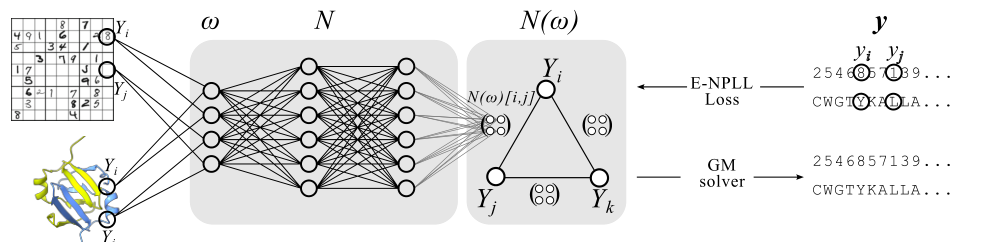
\includegraphics[width=11cm]{images/neuro_symbolic_architecture.png}
    \caption[Scaling Neuro-symbolic Problem Solving]{\textbf{Scaling Neuro-symbolic Problem Solving : Solver-Free Learning of Constraints and Objectives}.\cite{defresne_scaling_2026}}
\end{figure}

\begin{itemize}
    \item Raw inputs enter the neural network.
    \item The network predicts all pairwise cost functions.
    \item Toulbar2 computes the exact discrete output.
\end{itemize}

This effectively isolates perception from reasoning. It allows Toulbar2 to focus exclusively on the exact discrete optimization tasks where it dominates.

\subsection{Machine Learning Alternatives for Large Scale Optimization}

As established, Toulbar2 explores the whole solution space. This exploration makes it computationally infeasible for large scale constraint optimization problems. The application of modern artificial intelligence methods to directly address these specific limitations presents an interesting alternative.

Since Toulbar2 is too slow to generate optimal training labels for large instances, researchers have bypassed this limitation by utilizing self-supervised models like Deep Attentive Belief Propagation. This method infers optimal parameters dynamically without needing Toulbar2 to provide exact solutions.

We can also reduce communication overhead when integrating Toulbar2 with SAT solvers for \textit{Satisfiability Modulo Counting} (SMC\footnote{SMC (Satisfiability Modulo Counting) : combines logic rules with probability. It’s used in order to find answers that meet strict logical conditions and achieve a specific probability target.}). Traditional integrated systems run slowly due to continuous communication between the separate logic and probabilistic solvers, this problem is solved with integrated solvers like KOCO SMC\footnote{KOCO-SMC  is a SMC solver by tracking lower and upper bounds in the probabilistic inference process.}, they improve this by tracking lower and upper bounds during probabilistic inference. They also evaluate partial variable assignments early in order to help to prevent exhaustive enumerations.

\begin{figure}[H]
    \centering
    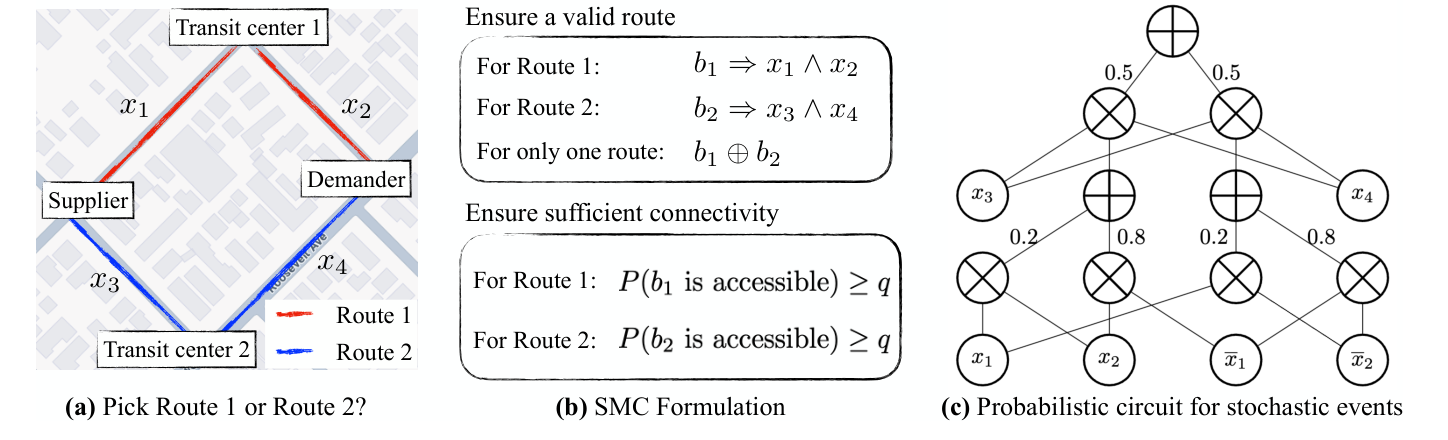
\includegraphics[width=11cm]{images/smc_example.png}
    \caption[Example of SMC : Robust Supply Chain with Different Network Size]{\textbf{Example of SMC : Robust Supply Chain with Different Network Size}.\cite{li_solving_2025}}
\end{figure}

\begin{figure}[H]
    \centering
    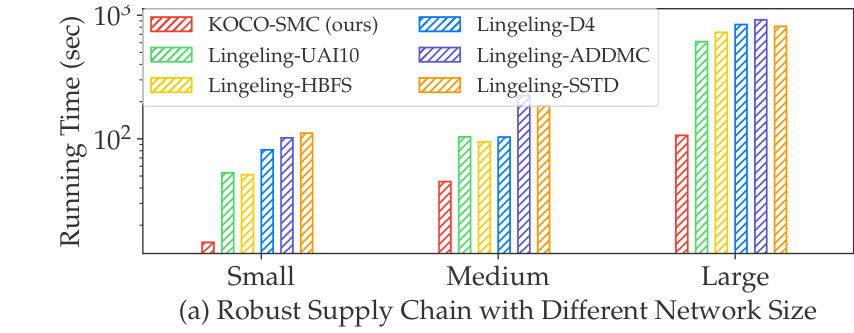
\includegraphics[width=9cm]{images/KOCO.png}
    \caption[Performance of each algorithm.]{\textbf{Performance of each algorithm.} Source \cite{li_solving_2025}}
\end{figure}

This algorithm is a significant improvement over previous systems like Lingeling-HBFS that rely on Toulbar2.

Artificial intelligence can additionally be utilized to match exact quality with linear scaling instead of exponential scaling Toulbar2 has. NeuroLifting addresses the limitations of Toulbar2 by using Graph Neural Networks to reparameterize decision variables. 
This transformation allows the optimization of models through standard gradient descent.
This method matches the solution quality of Toulbar2 on moderate scales and outperforms it on large problems due to linear computational growth.
\medskip{10cm}


The integration of artificial intelligence resolves the scaling limitations of the Toulbar2 in some problems.
Neural networks can also process the perception of the data to let the solver focus on discrete optimization tasks.
Emerging algorithms bypass exhaustive search through the application of gradient descent and dynamic probabilistic tracking.
This transition mandates that future solving methods rely on hybrid architectures rather than exact solvers.

\section{Conclusion}

The objective of this state-of-the-art review was to understand how a solver based on \ac{CFNs}, such as Toulbar2, established itself across such diverse disciplines. These fields range from structural biology to operations research and artificial intelligence. The answer lies in combining the expressiveness of the \ac{WCSP} formalism with the power of its local consistency algorithms (EDAC, VAC, OSAC).

The formalism can jointly model strict rules and preferences. Meanwhile, the algorithms efficiently prune complex combinatorial spaces.

This cross-analysis demonstrates that Toulbar2 has continuously evolved to adapt to the topology of these different problems. It first became essential in bioinformatics for processing dense molecular networks. It then proved its competitiveness in resource planning (both physical and human) by integrating sophisticated global constraints.

Today, facing the complexity of dynamic and uncertain environments, its role is transforming. It is no longer just a standalone tool. Instead, it hybridizes with probabilistic models to act as an exact inference engine within broader architectures. This natural evolution toward neuro-symbolic artificial intelligence redefines the role of exact methods.

It also raises new questions for future research. To what extent can constraint solvers like Toulbar2 be natively integrated into deep learning model training (Decision-Focused Learning) to correct their logical errors ? In the longer term, will we witness the emergence of a standardized hybrid AI ? In such a system, the lightning speed of neural perception and the mathematical optimality of \ac{CFNs} would become entirely inseparable.

\subsubsection*{Acknowledgements}
The authors would like to thank their research director, Martin Cooper, for his valuable guidance and support throughout this project.

\newpage
\section{Appendix}
\appendix

\section{List of Acronyms}

\begin{acronym}[MINLP]
    \acro{CSP}{Constraint Satisfaction Problem}
    \acro{WCSP}{Weighted Constraint Satisfaction Problem}
    \acro{VCSP}{Valued Constraint Satisfaction Problem}

    \acro{CFNs}{Cost Function Networks}
    \acro{EPTs}{Equivalence Preserving Transformations}
    \acro{SAC}{Soft Arc Consistency}
    \acro{FDAC}{Full Directional Arc Consistency}
    \acro{EDAC}{Existential Directional Arc Consistency}
    \acro{VAC}{Virtual Arc Consistency}
    \acro{OSAC}{Optimal Soft Arc Consistency}
    
    \acro{CP}{Constraint Programming}
    \acro{LP}{Linear Programming}
    \acro{ILP}{Integer Linear Programming}
    \acro{MILP}{Mixed-Integer Linear Programming}
    \acro{MINLP}{Mixed Integer Non-Linear Programming}
    \acro{MIP}{Mixed Integer Programming}

    \acro{KPCG}{knapsack problem with a conflict graph}
    
    \acro{SBF}{Smart Brute-force}
    \acro{MAP}{Maximum a Posteriori}
    \acro{ZP}{Zahn's problem}
    \acro{BnB}{Branch-And-Bound}

    \acro{CMD}{Computational Protein Design}
    \acro{PPI}{Protein–Protein Interactions}
    \acro{CPD}{Computer-aided Protein Design}
    \acro{GMEC}{Global Minimum Energy Conformation}
    \acro{LNS}{Large Neighborhood Search}
\end{acronym}

\section{Algorithms}

\subsection{MinCostMaxClique algorithm}

\begin{algorithm}[H]
    \caption{MinCostMaxClique}
    \label{algo:mcmc}
    
    \parbox{\linewidth}{
        \textbf{Where :} \\
        -- $p$, the number of aircraft \\
        -- Vect, a \textit{structure} representing a tuple of trajectories, and composed of an array \textit{tab} of size $p$, containing the id of nodes from the \textit{p}-partite graph ; an \textit{index} ; and a \textit{cost} \\
        -- $H$, a binary min heap of Vect sorted by their \textit{cost}
    }
    
    \vspace{0.3cm}
    \hrule
    \vspace{0.2cm}

    $\text{Vect}\, v; v'$\;
    $v.tab[0 .. p-1] := -1;\, v.index := 0$\;
    $v.tab[v.index]++$\;
    $H.insert(v)$\;
    \While{$H \text{ isn't empty}$}{
        $v := H.\textit{extract\_top}$\;
        \If{$v\, \textit{is legal}$}{
            \If{$v\,\textit{is solution}$}{
                \Return{$v$}\;
            }
            $v' := v$\;
            $v'.\textit{index}++;\, v'.tab[index]++$\;
            $H.insert(v')$\;
            $v.tab[index]++$\;
        }
        $H.insert(v)$\;
    }
    \Return{``No solution''}\;    
\end{algorithm}

% ==================================================================================================================================
% Biblio

\clearpage
%\printbibliography
\bibliographystyle{splncs04}
\nocite{*}
\bibliography{biblio}
\end{document}
